
\begin{figure}[H]
  \centering
  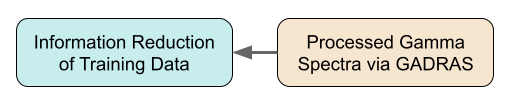
\includegraphics[width=0.7\linewidth]{./chapters/exp2/methodology2_2.png}
  \caption[Second portion of the flowchart from Figure \ref{fig:method2}]
          {Second portion of the flowchart from Figure \ref{fig:method2} being 
           described in this section.}
\end{figure}

The overall goal of this project is to determine how much information to what
quality is needed to train a  \gls{ML} model that can provide \gls{SNF}
attribution by correctly predicting the reactor type, burnup, \gls{U235}
enrichment, and time since irradiation.  In this section, the information
quality is treated as the information reduction (i.e. decreasing energy
resolution) of processed gamma spectra in the training database.  This
detector-based information reduction-focused treatment was not applied to the
mass measurements from the first experiment in Chapter \ref{ch:exp1} because
studying measurement techniques that can only be done in a lab is not the goal
of this work. \todo{check w/ paul -- trying to say I don't care about mass spec
errors and detection quality} Instead, field-deployable detectors are of
interest.

This process is outlined here for the second experiment, in which a gamma
spectrum is computed for each sample in the database from the nuclide
activities in Section \ref{sec:training2}.  The \gls{GADRAS} code \cite{gadras}
developed at Sandia National Laboratories will provide computational gamma
spectra.  This adds more than one layer of reduced information quality, which
are listed here, and also serve as an outline of the steps taken to process the 
gamma spectra:
\begin{enumerate}
  \item \label{itm:1} The list of nuclides is limited to manually chosen 
        radionuclides.
  \item \label{itm:2} Instead of "perfect" radionuclide activity knowledge, 
        they are being measured by a gamma detector.
  \item \label{itm:3} The processing of the gamma spectra can be highly variable.\todo{fix me}
  \item \label{itm:4} The $\sqrt{n}$ error of counts-based detection is included. 
\end{enumerate}

There is much ongoing work on the topic of attributing \gls{SNF} using gamma
detection using targeted or advanced measurement techniques \cite{snf_gamma,
compton_supp, bwr_high-res_gamma, pwr_bwr_gamma} and using innovative spectra
evaluation and radioisotope identification methods \cite{riid_09,
rapid_riid_18, sull_gen_07, sull_valid_15, sull_auto_17, sull_unc_17}.  Since
this is a topic of active research and the approaches are heavily
detector-dependent, a simple processing approach is described below.

\noindent \textbf{Step 1 : Choosing Radionuclides}

Step \ref{itm:1} is covered in Section \ref{sec:training2}.  

\noindent \textbf{Step 2: Computational Gamma Detection}

Step \ref{itm:2} refers to obtaining a gamma spectrum for every \gls{SNF} entry
in the database.  This is done using the \gls{GADRAS} tool, which applies a
\gls{DRF} to the gamma lines from these radionuclides. The input is a nuclide
activity vector, and the output is an array of energy bins (measured in $keV$),
and the counts per energy bin.

The nuclide activity data requires some processing to be used in this way.  The
activities that come from the \gls{ORIGEN} simulations are based on there being
$1\:MT$ of initial uranium-based fuel. Not only is this quantity an unlikely
amount to be smuggled, it would overwhelm a detector at the default/calibrated
source-detector distances in \gls{GADRAS}.  Therefore, the material (and
resulting nuclide activities) are scaled to be $1\:g$ of \gls{SNF}.

\todo[inline]{GADRAS overview here. also be clear about the required inputs and
what I gave for those inputs}

Regarding the input information for the \gls{GADRAS} calculations, the sources
are provided without any background; this is because any spectrum would undergo
background subtraction before further analysis. Additionally, the nuclides are
pre-decayed in \gls{ORIGEN} to correspond to various cooling times, but the
source age provided to \gls{GADRAS} needs to be a non-zero value. A source age
of $20\:minutes$ \todo{not super sensitive? tested this in 5 or 10 minute
steps?} provides the expected peaks.

\begin{table}[!htb]
  \centering
  \begin{tabular}{@{}lcllll@{}}
  \toprule
    \textbf{Detector} &
    \textbf{\begin{tabular}[c]{@{}c@{}}\% FWHM \\ @ 661 keV\end{tabular}} &
    \textbf{\begin{tabular}[c]{@{}l@{}}Distance \\ (cm)\end{tabular}} &
    \textbf{\begin{tabular}[c]{@{}l@{}}Height \\ (cm)\end{tabular}} &
    \textbf{\begin{tabular}[c]{@{}l@{}}Live Time\\ (s)\end{tabular}} &
    \textbf{\begin{tabular}[c]{@{}l@{}}Num \\ Channels\end{tabular}} \\ \midrule
    In-Lab HPGe           & 0.21 & 100.0 & 84.0  & 600  & 8192 \\
    Portable HPGe         & 0.29 & 100.0 & 100.0 & 600  & 8192 \\
    CZT                   & 1.20 & 100.0 & 100.0 & 600  & 1024 \\
    SrI\textsubscript{2}  & 2.94 & 100.0 & 100.0 & 600  & 1024 \\
    LaBr\textsubscript{3} & 3.63 & 213.0 & 84.5  & 2400 & 1024 \\
    NaI                   & 7.74 & 213.0 & 85.4  & 2400 & 1024 \\ \bottomrule
  \end{tabular}
  \caption[Details of detector setups]
          {Select details of 6 detector setups used to obtain gamma 
           spectra-based training databases.}
  \label{tbl:detsetups}
\end{table}

Training databases were created for the six detectors outlined in Table
\ref{tbl:detsetups}. They were chosen to compare the highest energy resolution
detector, a lab-based \gls{HPGe}, against the rest, in order of decreasing
energy resolution: portable \gls{HPGe}, \gls{CZT}, \gls{SrI2}, \gls{LaBr3}, and
\gls{NaI} detectors. This is displayed in the table by including the \gls{FWHM}
of the $661\:keV$ peak for ${}^{137}\text{Cs}$. At this point, there are six
versions of the original database for each detector setup, but there is a full
gamma spectrum for each \gls{SNF} entry.\todo{fix confusing sentence} It is not
computationally prudent to use full gamma spectra for training and testing,
since the spectra returned have 1024 or 8192 bins, and machine learning
algorithms are not designed to handle thousands of features.  Thus, these
spectra are processed; this is step \ref{itm:3} from above, and is outlined as
follows.

\noindent \textbf{Step 3: Processing Gamma Spectra}

Step \ref{itm:3} covers the steps taken to process the gamma spectrum generated
for each \gls{SNF} entry into a training set where the features are now summed
windows of a range of energy bins.\todo{be clear about why this choice makes
sense}  There are two main design choices here: the width of the energy windows
and the number of energy windows to include. The energy window width is a value
that was manually chosen \todo{say how you chose the window size clearly} and
does not change for each detector.  The different energy window widths are
listed in Table \ref{tbl:enwindows}.

\begin{table}[!htb]
  \centering
  \begin{tabular}{@{}lcm{0.7in}m{0.7in}m{0.7in}@{}}
    \toprule
    \multirow{2}{*}{\textbf{Detector}} &
    \multirow{2}{*}{\textbf{\begin{tabular}[c]{@{}l@{}}Energy Window\\ Size {[keV]}\end{tabular}}} &
    \multicolumn{3}{c}{\textbf{\# of Energy Windows}} \\ \cmidrule(l){3-5}
                     &    & Auto & Short & Long \\
    \toprule
    In-Lab HPGe      & 2  & 206  & 42    & 151  \\
    Portable HPGe    & 3  & 120  & 42    & 151  \\
    CZT              & 8  & 30   & 42    & 151  \\
    $\text{SrI}_2$   & 10 & 17   & 42    & 151  \\
    $\text{LaBr}_3$  & 12 & 19   & 42    & 151  \\
    NaI              & 12 & 9    & 42    & 151  \\ 
    \bottomrule
  \end{tabular}
  \caption[Energy window sizes and list lengths for processing gamma spectra]
          {Energy window sizes and list lengths for 6 detector setups used to 
           process the gamma spectra-based training databases.}
  \label{tbl:enwindows}
\end{table}

Table \ref{tbl:enwindows} lists three energy window list length columns,
\textit{Auto}, \textit{Short}, and \textit{Long}. These correspond to different
processed training sets that have a different number of energy windows
included.  There are two approaches taken: a nuclear physics-based method that
generates an energy window list based on the gamma energies expected to be
detected (short and long), and an automatic peak search of a manually chosen
gamma spectrum in the full gamma spectra training database (auto). 

The first method creates the short and long lists in Table \ref{tbl:enwindows};
the length of these lists are the same for all detectors because they are based
on the gamma energies most likely to be detected, which is independent of the
detector quality. To obtain these lists, the expected number of decays of each
gamma energy is calculated based on the activities of the 32 tracked nuclides
using the Python for Nuclear Engineering toolkit \cite{pyne} from a reference
sample in the training set.  This reference sample emerged as the sample of
choice because it contains the superset of gamma energies of all tested
samples, of which there were nine (three for each reactor type).

After the expected number of decays for each gamma energy for all 32 nuclides
are calculated, an arbitrary minimum number of decays is selected to filter out
the gamma energies that are unlikely to produce counts high enough to be
detected. The first arbitrary minimum number of decays is set at $5 \times
10^8$ decays, and the long list of 151 gamma energies that remain above this
cutoff is created.  A list of length 151 is likely to contain many features
that do not contribute discrimination to the models, and thus they may add
noise to the training set, so a shorter list is needed.  So, a higher arbitrary
minimum of $5 \times 10^{10}$ decays is chosen; this threshold creates the
short list of 42 gamma energies. 

The short and long lists of gamma energies correspond to the nuclides in Table
\ref{tbl:enlistnucs}. The 12 nuclides listed come from the long list, and the
subset of seven bold nuclides come from the short list.  To determine a "full
knowledge" scenario for the detector-based training sets, two training sets are
also created with the 7- and 12-nuclide activity lists.  It should be noted
that several (three for each reactor type) training set entries were selected
based on sampling evenly throughout the training set parameters, with the
intention that there would be a set of gamma energies comprised from multiple
entries. However, one sample emerged as a superset of the others. This sample
is thus chosen for the second method, discussed next.

\begin{table}[!htb]
  \centering
  \begin{tabular}{@{}|l|l|l|@{}}
    \hline
    \allbold{${}^{241}\text{Am}$} & \allbold{${}^{243}\text{Am}$} & ${}^{243}\text{Cm}$           \\ \hline
    ${}^{244}\text{Cm}$           & ${}^{245}\text{Cm}$           & \allbold{${}^{134}\text{Cs}$} \\ \hline
    \allbold{${}^{137}\text{Cs}$} & ${}^{152}\text{Eu}$           & \allbold{${}^{154}\text{Eu}$} \\ \hline
    \allbold{${}^{85}\text{Kr}$}  & ${}^{238}\text{Pu}$           & \allbold{${}^{125}\text{Sb}$} \\ \hline
  \end{tabular}
  \caption[Nuclides that are represented by the short and long energy windows 
           lists]
          {Nuclides that are represented by the gamma energy lines in the 
           energy lists. The entire set of 12 nuclides belongs to the long 
           list, and the 7 bold nuclides belong to the short list.}
  \label{tbl:enlistnucs}
\end{table}

The column denoted as \textit{Auto} in Table \ref{tbl:enwindows} is obtained by
a physics-free approach. It is based on a peak search of a spectrum in the full
gamma spectra training database. The previously mentioned sample is selected
for all six detectors, and a peak searching algorithm implemented in python
using the SciPy toolkit \cite{scipy} is applied. Using the peak search on the
six different spectra for the same sample, the resulting number of energy
windows for each detector is in Table \ref{tbl:enwindows}.  

%this is idx 66796
\begin{figure}[!htb]
  \makebox[\textwidth][c]{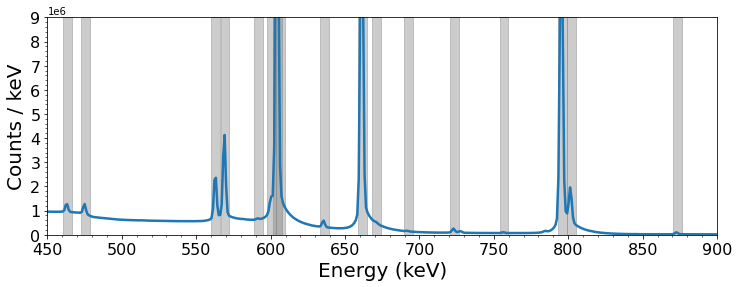
\includegraphics[width=\linewidth]{./chapters/exp2/energy_window_example.png}}
  \caption[Portion of gamma spectrum with windows, which shows summation regions 
           for spectra processing]
          {Slice of an example gamma spectrum in one of the training databases
           showing the windows over the gamma energy peaks. This is the portable
           \acrshort{HPGe} with the auto energy window list and the reference 
           sample's spectrum.}
  \label{fig:enwindows}
\end{figure}

After the three energy window lists are created, the full gamma spectra are
processed into three training sets, one for each list.  The energy window width
for each detector is used to sum the binned counts for each list entry; that
is, the counts are summed for each gamma energy in the list $\pm E_{width}$.
This is visualized in Figure \ref{fig:enwindows}, where a portion of a portable
\gls{HPGe} spectrum is shown with the $\pm3\:keV$ windows from the auto energy
window list.  Three training sets are created for each detector, resulting in
18 detector-based processed gamma spectra training sets.

\noindent \textbf{Step 4: Apply Statistical Counting Error}

Lastly, step \ref{itm:4} involves the inclusion of the counting error for the
summed energy windows. This is quite simple, as statistical counting error of
$n$ counts is $\sqrt{n}$.  As in Section \ref{sec:inforeduc1}, this error gets
applied in the same way for the scikit-learn algorithms, where the uniform
error is applied randomly within the range $[x_i - \sqrt{x_i}, x_i +
\sqrt{x_i}]$ for each summed energy window $x_i$. For the \gls{MLL}
calculations, Equation \ref{eq:mllunc} is used, where $\sigma_{i} =
\sqrt{x_i}$.  
